%%%%%%%%%%%%%%%%% (2023) Fraga & Silva Neto.tex %%%%%%%%%%%%%%%%%%%
%
% Article in preparation by Fraga (2023).
%
% Please cite this paper as an work in progress.
% Respect the license presented in the README.me file.
%
%%%%%%%%%%%%%%%%%%%%%%%% Springer-Verlag %%%%%%%%%%%%%%%%%%%%%%%%%%
%
% First comes an example EPS file -- just ignore it and
% proceed on the \documentclass line
\begin{filecontents*}{example.eps}
%%CreationDate: Mon Fev 06 2023
%%Creator: Tatiana Balbi Fraga
%%EndComments
gsave
newpath
  20 20 moveto
  20 220 lineto
  220 220 lineto
  220 20 lineto
closepath
2 setlinewidth
gsave
  .4 setgray fill
grestore
stroke
grestore
\end{filecontents*}
%
% Choose either the first of the next two \documentclass lines for one
% column journals or the second for two column journals.
% Make sure that meanwhile no specific package for your very project has
% appeared by viewing the web page
% http://www.springer.de/author/tex/help-journals.html
\documentclass[global,referee]{svjour}
%\documentclass[global,twocolumn,referee]{svjour}
% Remove option referee for final version
%
% Remove any % below to load the required packages
%\usepackage{latexsym}
\usepackage{graphics}

\usepackage{tikz}
\usetikzlibrary{shapes.geometric, arrows}

\tikzstyle{none} = [rectangle, 
minimum width=0cm, 
minimum height=0cm,
text centered]

\tikzstyle{operation} = [rectangle, 
minimum width=3cm, 
minimum height=1cm,
text centered, 
draw=black, 
fill=black!15]

\tikzstyle{finalOperation} = [rectangle, rounded corners, text width=2.5 cm,
minimum width=3cm, 
minimum height=1cm,
text badly centered, 
draw=black, 
fill=black!25]

\tikzstyle{result} = [rectangle, rounded corners, 
minimum width=3cm, 
minimum height=1cm,
text centered, 
draw=black, 
fill=black!25]

\tikzstyle{question} = [ellipse, text width=3cm,
minimum width=3cm, 
minimum height=1cm,
text centered, 
draw=black, 
fill=black!05]

\tikzstyle{answer} = [diamond, text width=1cm,
minimum width=1cm, 
minimum height=1cm,
text centered, 
draw=black, 
fill=black!35]

\tikzstyle{line} = [thick,-,>=stealth]
\tikzstyle{arrow} = [thick,->,>=stealth]


% etc
%
% Insert the name of "your" journal with the command below:
\journalname{Brazilian Journal of Systems Analysis, Modeling and Optimization}
%
\begin{document}
%
\title{Similar Particle Collision for the Job Shop Scheduling Problem}
%\subtitle{Do you have a subtitle?\\ If so, write it here}
\author{Tatiana Balbi Fraga\inst{1} \and Antonio Jose da Silva Neto\inst{2}% etc
% \thanks is optional - remove next line if not needed
\thanks{\emph{Present address:} Insert the address here if needed}%
}                     % Do not remove
%
\offprints{}          % Insert a name or remove this line
%
\institute{Centro Acadêmico do Agreste / Universidade Federal de Pernambuco \and Instituto Politécno do Rio de Janeiro / Universidade Estadual do Rio de Janeiro}
%
\date{Received: date / Revised version: date}
% The correct dates will be entered by the editor
%
\maketitle
%
\begin{abstract}
In this paper we present the Similar Particle Collision heuristic (SPC) and the Similar Particle Multicollision algorithm with Exploration by Tabu Search, specially developed to solve the Job Shop Scheduling Problem. Although there is a wide range of heuristics and algorithms developed to solve this famous problem, the SPC has an interesting characteristic, since its application is not very sensitive to the adjustment of the parameters used. Another important characteristic is that the presented heuristic allows the successful hybridization of different algorithms mixing aspects of local and global exploration. As we can see, the results are as good as the best results presented in the literature and the method attenuates the different results found by adjusting the parameters, leading to a more robust search.
\end{abstract}
%
\section{Introduction}
\label{intro}

08/02/2023 - 7:21 - starting a new working day

Talk about heuristics for combinatorial optimizatiom problem and hibridization.

\subsection{Job Shop Scheduling Problem}
\label{sec:JSSP}

Present the Job Shop Scheduling problem. 
Lecture on the algorithms applied to solve the problem and in particular on hybrid algorithms.


\subsection{Particle Collision method}
\label{sec:PC}

By observing the physics of the collision process between nuclear particles inside a nuclear power reactor it is possible to verify that, among the colliding particles, those that reach the nuclei, i.e. regions of high fitness, are absorbed and explore the surroundings while that those that reach regions of low fitness can be absorbed or spread to other regions according to some probability function. Analyzing these interactions, Sacco and Oliveira (2005) observed that the succession of absorption and scattering events allowed the movement of particles to promote an exploration of the complete search space while a deeper exploration of the most promising areas. Thus, based on this observation, the authors proposed a new algorithm for search which they named the Particles Collision Algorithm. In this algorithm initially a solution is chosen and reserved as current solution. Then, this current solution is perturbed through a Perturbation() function, generating a new solution. If the new solution is “better” than the current solution (according to some previously defined criteria), the last solution is replaced by the first and on this a local search procedure defined by an Exploration() function is applied. If the new solution is “worse” than the current solution, then a function Scatter() is applied, where a probability function is used to define whether the current solution will be explored or replaced by a random solution. Note that this algorithm has a similar structure to Simulated Annealing except for the fact that the algorithm can be taken to new search spaces not directly related to the initial solution. Additionally, it is not necessary to define an initial temperature. Fig. 1 presents a pseudo-code for the PCA, as proposed by Sacco et al. (2006) for solving continuous maximization problems. Note that the function of probability is defined by the criterion of Metropolis (METROPOLIS et al., 1953). 

%Fig. 2 and 3 present, respectively, the %functions Disturbance() and Small_Diturbance()

applied in the same algorithm. In these figures it is possible to observe that, when working with continuous variable problems, perturbations are generated through variations random changes in the value of each variable within previously established limits, with the small perturbations similar to the perturbations, differing only in the limits that are more narrow. In the case of discrete problems like PEPOM, it is necessary to define how these disturbances will take place. 

Than inform what subject is discussed in this paper and highlight the innovative aspects of the work

\section{Similar Particle Collision heuristic}
\label{sec:SPC}

In Similar Particle Collision heuristic (Fig. \ref{fig:PCH}) the functions, Disturbance() and Exploit() are respectively replaced by operators of Disturbance and Local Exploration. As Disturbance operators, whose purpose is to take the algorithm to new search spaces, we sugest mutation operators used in Genetic Algorithms, such as the operators M1 to M10 presented by Lian et al. (2006). Alternatively, if the Similar Particle Collision algorithm is applied simultaneously to all individuals of an initial population, we sugest crossover operators used in Genetic Algorithms, applied on pairs of solutions, such as the operators C1 to C4 also presented by Lian et al. (2006). In the case of Local Exploration operators, whose purpose is to explore the surroundings of a given solution, we suggest the various local search algorithms built based on heuristics such as Simulated Annealing, Genetic Algorithms, Particle Collision and Tabu Search. \\

\begin{figure}
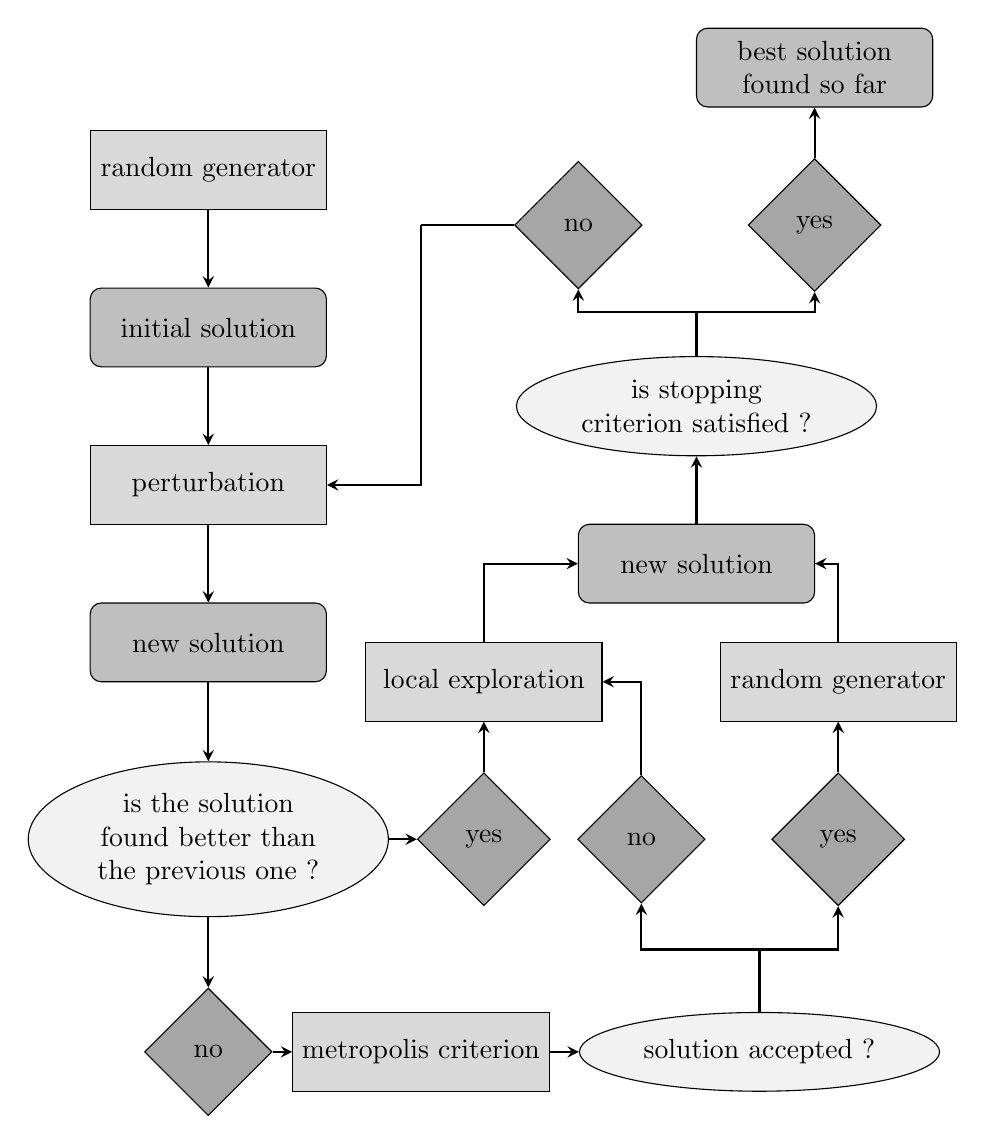
\begin{tikzpicture}[node distance=2cm]
\node (random) [operation] {random generator};
\node (inSol) [result, below of=random] {initial solution};
\node (perturbation) [operation, below of=inSol] {perturbation};
\node (newSol) [result, below of=perturbation] {new solution};
\node (q1) [question, below of=newSol, yshift=-0.5cm] {is the solution found better than the previous one ?};
\node (a11) [answer, below of=q1, yshift=-0.7cm] {no};
\node (met) [operation, right of=a11, xshift= 0.7 cm] {metropolis criterion};
\node (q2) [question, right of=met, xshift= 2.3 cm] {solution accepted ?};
\node (q21) [none, above of=q2, yshift=-0.7cm] {};
\node (a21) [answer, above of=q2, xshift=-1.5 cm, yshift= 0.7cm] {no};
\node (a22) [answer, above of=q2, xshift= 1.0 cm, yshift= 0.7cm] {yes};
\node (newRandom) [operation, above of=a22] {random generator};
\node (a12) [answer, right of=q1, xshift= 1.5 cm] {yes};
\node (lcExp) [operation, above of=a12] {local exploration};
\node (newNewSol) [result, above of=lcExp, xshift= 2.7 cm, yshift= -0.5 cm] {new solution};
\node (q3) [question, above of=newNewSol] {is stopping criterion satisfied ?};
\node (q31) [none, above of=q3, yshift=-0.8cm] {};
\node (a31) [answer, above of=q3, xshift=-1.5 cm, yshift= 0.3 cm] {no};
\node (a311) [none, left of=a31] {};
\node (a32) [answer, above of=q3, xshift= 1.5 cm, yshift= 0.3 cm] {yes};
\node (stop) [finalOperation, above of=a32] {best solution found so far};


\draw [arrow] (random) -- (inSol);
\draw [arrow] (inSol) -- (perturbation);
\draw [arrow] (perturbation) -- (newSol);
\draw [arrow] (newSol) -- (q1);
\draw [arrow] (q1) -- (a11);
\draw [arrow] (a11) -- (met);
\draw [arrow] (met) -- (q2);
\draw [line] (q2.north) -- (q21.center);
\draw [arrow] (q21.center) -| (a21.south);
\draw [arrow] (a21.north) |- (lcExp);
\draw [arrow] (q21.center) -| (a22.south);
\draw [arrow] (a22) -- (newRandom);
\draw [arrow] (q1) -- (a12);
\draw [arrow] (a12) -- (lcExp);
\draw [arrow] (lcExp.north) |- (newNewSol);
\draw [arrow] (newRandom.north) |- (newNewSol);
\draw [arrow] (newNewSol) -- (q3);
\draw [arrow] (q31.center) -| (a31.south);
\draw [line] (a31) -- (a311.center);
\draw [arrow] (a311.center) |- (perturbation.east);
\draw [line] (q3) -- (q31.center);
\draw [arrow] (q31.center) -| (a32);
\draw [arrow] (a32) -- (stop);
\end{tikzpicture}
\caption{Particle Collision Heuristic.}
\label{fig:PCH}  
\end{figure}


\section{Similar Particle Multicollision algorithm with Exploration by Tabu Search}
\label{sec:SPCETS}

Include explanation about the algorithm
and \cite{RefJ}

\section{Tests and results}
\label{sec:results}

~\ref{sec:1}.

\section{Conclusions and future work}
\label{sec:conclusions}

%
% For one-column wide figures use
\begin{figure}
% Use the relevant command for your figure-insertion program
% to insert the figure file.
% For example, with the option graphics use
%\resizebox{0.75\textwidth}{!}{%
%  \includegraphics{example.eps}
%}
% If not, use
%\vspace{5cm}       % Give the correct figure height in cm
\caption{Please write your figure caption here}
\label{fig:1}       % Give a unique label
\end{figure}
%
% For two-column wide figures use
\begin{figure*}
% Use the relevant command for your figure-insertion program
% to insert the figure file. See example above.
% If not, use
\vspace*{5cm}       % Give the correct figure height in cm
\caption{Please write your figure caption here}
\label{fig:2}       % Give a unique label
\end{figure*}
%
% For tables use
\begin{table}
\caption{Please write your table caption here}
\label{tab:1}       % Give a unique label
% For LaTeX tables use
\begin{tabular}{lll}
\hline\noalign{\smallskip}
first & second & third  \\
\noalign{\smallskip}\hline\noalign{\smallskip}
number & number & number \\
number & number & number \\
\noalign{\smallskip}\hline
\end{tabular}
% Or use
\vspace*{5cm}  % with the correct table height
\end{table}
%
% BibTeX users please use
% \bibliographystyle{}
% \bibliography{}
%
% Non-BibTeX users please use
\begin{thebibliography}{}
%
% and use \bibitem to create references.
%
\bibitem{RefJ}
% Format for Journal Reference
Author, Journal \textbf{Volume,} (year) page numbers.
% Format for books
\bibitem{RefB}
Author, \textit{Book title} (Publisher, place year) page numbers
% etc
\end{thebibliography}


\end{document}

% end of file template.tex

